% ROCS 2026 short paper (4 pages + references), IEEEtran conference, 10 pt.
% Plan, budgets and writing rules: v2/paper/PAPER_PLAN.md.
% Tables/figures: \input / \includegraphics from ../generated/ (make_all.py output, gitignored);
% run `.venv/bin/python v2/paper/scripts/make_all.py` before building.
% Numbers in the prose carry a "% src:" comment naming the results CSV (or generated table) they come from.
\documentclass[conference,10pt]{IEEEtran}
\IEEEoverridecommandlockouts
\usepackage{cite}
\usepackage{amsmath,amssymb}
\usepackage{graphicx}
\usepackage{booktabs}
\usepackage{url}
\usepackage{xspace}
\usepackage{tikz}
\usetikzlibrary{positioning}

\graphicspath{{../generated/}}
\newcommand{\ceil}[1]{\left\lceil #1 \right\rceil}
\newcommand{\cpipe}{C_{\mathrm{PIPE}}}
\newcommand{\cstart}{C_{\mathrm{START}}}
\newcommand{\kvtsx}{KV260\xspace}

\begin{document}

% TODO title: pick one of the three working titles in PAPER_PLAN.md.
\title{Predictable by Construction: A Cycle-Exact, Bit-Exact INT8 CNN Accelerator on the Kria KV260}

% TODO authors
\author{\IEEEauthorblockN{TODO Author}
\IEEEauthorblockA{TODO Affiliation\\ TODO email}}

\maketitle

% Abstract + Section I. Budgets: abstract 0.4 col (~180 words), intro 0.8 col (PAPER_PLAN.md).
\begin{abstract}
FPGA accelerator papers often report performance from models or simulation,
leaving the gap to real hardware unquantified. We present an INT8 CNN
accelerator for the AMD Kria KV260 whose performance is exactly predictable.
An $8{\times}8$ output-stationary array of DSP48E2 slices runs LeNet-5 and a
CIFAR-10 network entirely on chip at 250\,MHz, using 80 DSPs and 16.5k LUTs.
Its integer requantization reproduces the floating-point reference on every
non-saturating input of every channel. An analytical cycle model, fixed
before RTL simulation, predicts every layer's cycle count with zero error on
20,000 test images and 286 random layer configurations, in RTL simulation
and on the board. Measured on the KV260, accelerator compute takes 65.7\,$\mu$s
(LeNet-5) and 417.0\,$\mu$s (CIFAR-10) with a single cycle count over 3.65M
inferences, and 0.065 and 0.161\,mJ per image of SOM-rail energy. End to
end through a Python host it is 2.1--3.1$\times$ faster than the best
on-board Cortex-A53 baseline; against the AMD DPU it is 1.5$\times$ faster on
LeNet-5 and 1.6$\times$ slower on CIFAR-10. All results are regenerated by
script from a tagged commit.
\end{abstract}
% src: tab_t1_impl (80 DSP, 16,538 LUT @250); tab_layer_spread / tab_shapes (board, cycle-exact);
% tab_soak (3,651,181 jobs, 1 distinct TOTAL_CYC); tab_a5_cpu (65.7 / 417.0 us; speedups 3.10x / 2.11x;
% DPU/accel e2e 1.54x / 0.61x); tab_b1_power (E_sys 0.065 / 0.161 mJ).

\section{Introduction}\label{sec:intro}
FPGA CNN accelerators are usually evaluated with an analytical model or a
simulator, and the design that reaches the board is then characterized by
a few throughput figures. How far the model is from the hardware, layer by
layer, is rarely reported. That gap matters for two reasons. Embedded and
real-time systems need latency they can budget for, not latency that is
usually close. And a performance model is only useful for design-space
exploration if it can be trusted without building every design.

This paper takes the opposite route to the usual one. We wrote the cycle
model first, derived its two constants from the RTL's stage latencies and
committed them before the first simulation of the core, and then held the
RTL and the board to that model cycle for cycle. The design is deliberately
small: one $8{\times}8$ INT8 array on the AMD Kria KV260, all weights in BRAM,
and two small networks. Our claim is exactness and determinism, not peak
throughput, and we compare it honestly with the CPU and the vendor DPU on
the same board. Our contributions are:
\begin{itemize}
\item An $8{\times}8$ output-stationary INT8 accelerator on the KV260 whose
integer requantization is checked bit-exact against the floating-point
reference on every non-saturating input of every channel
(Secs.~\ref{sec:arch}, \ref{sec:verif}).
\item A closed-form cycle model, with constants fixed before RTL simulation,
that predicts every layer's cycles exactly on 20,000 test images, 286 random
layer jobs and the board (Secs.~\ref{sec:model}, \ref{sec:results}).
\item A board evaluation on the same KV260: deterministic compute latency,
SOM-rail energy, a 7-point clock sweep, and a comparison with the on-board
Cortex-A53 and the AMD DPU (Sec.~\ref{sec:results}).
\item A reproducible artifact: every reported number is generated by script
from a tagged commit, with hashed logs and bitstreams.
\end{itemize}

% Section II -- Related work (target 120 words).
% Writing rule 6: every cited paper must be read by a team member before submission
% (status in v2/paper/RELATED_NOTES.md -- none ticked yet).
\section{Related Work}\label{sec:related}
Dataflow taxonomies trade data reuse against utilization~\cite{sze2017efficient}.
FPGA designs choose their tiling from roofline or loop-optimization
models~\cite{zhang2015optimizing,ma2018optimizing}, stream binarized networks
through per-layer pipelines~\cite{umuroglu2017finn}, or run compiled
instructions on embedded Zynq devices~\cite{guo2018angeleye}; our numerics
follow integer-only quantization~\cite{jacob2018quantization}.
Timeloop~\cite{parashar2019timeloop}, MAESTRO~\cite{kwon2019maestro} and
SCALE-Sim~\cite{samajdar2020scalesim} model performance across large design
spaces, and Gemmini~\cite{genc2021gemmini} shows that system effects outside the
accelerator change measured results, as our host-side latency also shows. The AMD DPU~\cite{amd_pg338} is the standard CNN engine on
Kria devices~\cite{costa2026kv260}; we use it as a same-board baseline. We are
not aware of work in which an analytical model, RTL simulation and board
measurements agree exactly on every layer.

% Section III -- Architecture (target 380 words) + Fig. 1 (TikZ).
% Spec of record: v2/docs/ARCH_SPEC.md (frozen), v2/docs/FORMATS.md, DECISIONS D1/D2/D8/D13.
\section{Architecture}\label{sec:arch}
% Fig. 1 -- accelerator block diagram (TikZ, single column). Structure per v2/docs/ARCH_SPEC.md.
\begin{figure}[t]
\centering
\resizebox{\columnwidth}{!}{%
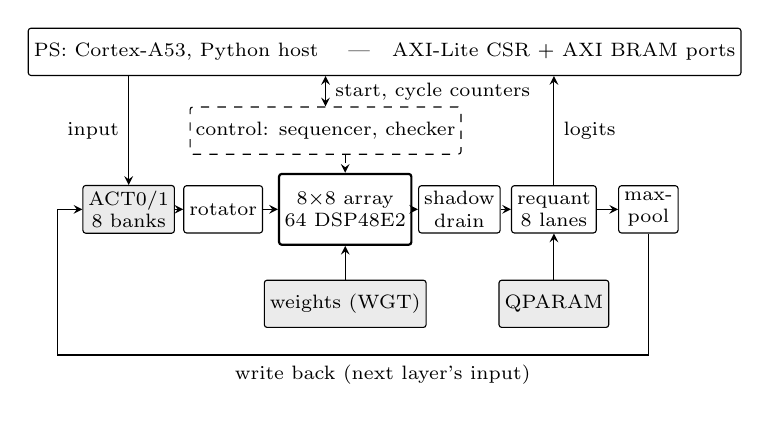
\begin{tikzpicture}[font=\scriptsize, >=stealth,
  blk/.style={draw, rounded corners=1pt, align=center, inner sep=2pt, minimum height=6mm},
  mem/.style={blk, fill=black!8},
  ctl/.style={blk, dashed}]
  % PS
  \node[blk, minimum width=7.9cm] (ps) at (-0.3,2.75)
      {PS: Cortex-A53, Python host \quad|\quad AXI-Lite CSR + AXI BRAM ports};
  % datapath (one row, left to right)
  \node[mem] (act)  at (-3.55,0.75) {ACT0/1\\8 banks};
  \node[blk] (rot)  at (-2.35,0.75) {rotator};
  \node[blk, line width=0.8pt, minimum height=9mm] (arr) at (-0.8,0.75) {$8{\times}8$ array\\64 DSP48E2};
  \node[blk] (drn)  at (0.65,0.75) {shadow\\drain};
  \node[blk] (rq)   at (1.85,0.75) {requant\\8 lanes};
  \node[blk] (pool) at (3.05,0.75) {max-\\pool};
  % memories and control (second row)
  \node[mem] (wgt) at (-0.8,-0.45) {weights (WGT)};
  \node[mem] (qp)  at (1.85,-0.45) {QPARAM};
  \node[ctl] (seq) at (-1.05,1.75) {control: sequencer, checker};
  % data flow
  \draw[->] (act) -- (rot);
  \draw[->] (rot) -- (arr);
  \draw[->] (arr) -- (drn);
  \draw[->] (drn) -- (rq);
  \draw[->] (rq) -- (pool);
  \draw[->] (wgt) -- (arr);
  \draw[->] (qp) -- (rq);
  \draw[->] (pool.south) -- (3.05,-1.1) -- (-4.45,-1.1) node[pos=0.45, below] {write back (next layer's input)} -- (-4.45,0.75) -- (act.west);
  \draw[dashed,->] (seq.south -| arr.north) -- (arr.north);
  % host interface
  \draw[->] (act.north |- ps.south) -- (act.north) node[pos=0.5, left] {input};
  \draw[<->] (seq.north |- ps.south) -- (seq.north) node[midway, right] {start, cycle counters};
  \draw[->] (rq.north) -- (rq.north |- ps.south) node[midway, right] {logits};
\end{tikzpicture}}
\caption{Accelerator organization. Weights and activations stay in BRAM; the host writes the input,
starts a job and reads the logits and cycle counters.}
\label{fig:arch}
\end{figure}


\textbf{Numeric contract.} Activations and weights are signed INT8 with
zero-point 0, a per-tensor activation scale and per-output-channel weight
scales; products accumulate in INT32. Each output channel stores
$(q_b, m, s)$: $v = \mathit{acc} + q_b$ is multiplied by the unsigned 32-bit
$m$, shifted right by $s$ with round-half-to-even, then passed through ReLU
and clipped to INT8. % src: ARCH_SPEC.md "Hardware requant"; B = 32 (DECISIONS D1 outcome)
The final layer exports raw INT32 logits, and the host applies the
reference's float32 dequantization and argmax.

\textbf{Datapath.} The core is an $8{\times}8$ output-stationary array of
DSP48E2 slices (Fig.~\ref{fig:arch}). Rows hold 8 consecutive output pixels
of one row and columns hold 8 output channels. Every cycle the array
consumes one reduction index $k = (ic, k_y, k_x)$: 8 activations and 8
weights are broadcast without skew, and the first product of a tile
overwrites the accumulator, so no clear cycle is needed. At the end of a
tile the 64 accumulators move to shadow registers, which drain one output
channel per cycle while the next tile accumulates. Eight requantization
lanes and a fused, bypassable $2{\times}2$ max-pool follow.
% src: ARCH_SPEC.md Datapath

\textbf{Memory.} Nothing leaves the chip during inference. Two ping-pong
activation buffers of 8 byte-wide banks hold a layer's input and output; a
pixel at column $x$ lives in bank $x \bmod 8$. For kernel offset $k_x$,
bank $b$ supplies output row $(b - k_x) \bmod 8$ and a byte rotator restores
the order, so all 8 operands arrive in one cycle without conflicts. All
weights stay resident in a 64-bit-wide weight memory.
% src: ARCH_SPEC.md Memory

\textbf{Control and interface.} Addresses come from counters and additions
only; the host precomputes derived fields in a 16-word descriptor per layer.
Data and control travel together as tokens through the pipeline, so no
stage infers timing by counting cycles. A sequencer runs up to 8 layers per
start, and a pipelined checker refuses illegal descriptors with an error
code before any work starts. % src: ARCH_SPEC.md Controller; DECISIONS D8-1, D13
The PS sees an AXI-Lite register file with 64-bit total-cycle, MAC-active
and stall counters, per-layer cycle counters, 16 logit registers and a
BUILD\_ID; the design loads as a PYNQ overlay. % src: ARCH_SPEC.md CSR
Of its 16,538 LUTs, the core uses 3,338; the rest is the AXI shell
(Table~\ref{tab:impl}). % src: tab_impl_compact (CLB LUT 16,538 / 3,338)

\textbf{Supported layers.} VALID convolutions with stride~1, optional ReLU
and $2{\times}2$ max-pooling; fully connected layers run as $1{\times}1$
convolutions on a $1{\times}1$ map. Kernel width is limited to 9 by the
rotator, a limit the host enforces (Sec.~\ref{sec:verif}).
% src: ARCH_SPEC.md Workloads; DECISIONS OC-3 (MAX_KW = 9)

% Section IV -- Cycle model. Budget: 0.6 columns (PAPER_PLAN.md).
% Sources: v2/model/gos_cycle_model.py, DECISIONS D10-8 / D13, cycle_model.csv,
% utilization_model.csv, schedule_ablation.csv (all model), tab_a3_cycles / tab_a4_util.
\section{Cycle Model}\label{sec:model}

Because the array accepts one reduction index per cycle and never stalls, a
layer's cost follows from its loop nest alone. Tiles iterate over output-channel
groups, output rows and 8-wide output column groups, giving
\begin{equation}
T = \ceil{OC/8} \cdot OH \cdot \ceil{OW/8}, \qquad K = IC \cdot KH \cdot KW .
\end{equation}
Each tile streams $K$ cycles, and the drain of one tile hides under the next
tile's accumulation. A layer therefore takes
\begin{align}
\mathit{LAYER\_CYC} &= T K + \cpipe, \label{eq:model}\\
\mathit{TOTAL\_CYC} &= \cstart + \textstyle\sum_{\text{layers}} \mathit{LAYER\_CYC},\nonumber
\end{align}
where $\cpipe = 29$ is the fill and flush latency of the token pipeline (sum of
the stage latencies from descriptor load to the last write) and $\cstart = 3$
is the pipelined descriptor check. % src: DECISIONS D10-8 (C_PIPE = 29 breakdown), D13 (C_START = 3)
Both constants were derived from the RTL's stage latencies and committed
before any simulation of the core; a unit test ties every term to the RTL
parameters. RTL simulation then matched without correction.
% src: DECISIONS D10-8 (commit 1eb0873), D13 (commit 04470fc)
For the two networks, (\ref{eq:model}) gives 16,436 and 104,247 cycles per
image (model), or 65.7 and 417.0\,$\mu$s at 250\,MHz;
Sec.~\ref{sec:results} compares these with RTL simulation and the board.
% src: cycle_model.csv / tab_a3_cycles.tex Total row; tab_a2_latency.tex 250 MHz row (65.74 / 416.99 us); PAPER_PLAN final numbers 65.7 / 417.0 us

\textbf{Utilization.} The array holds a valid input on 99.10\,\% (LeNet-5) and
99.89\,\% (CIFAR-10) of all cycles; only the $\cpipe$ fill is idle (model, equal
in RTL simulation). % src: tab_a4_util.tex Total "Array busy fraction" Model/RTL
Useful MACs per available PE-cycle are lower: 39.6\,\% and 67.3\,\% (model).
% src: utilization_model.csv total rows util_total 0.395968 / 0.673497
Partial 8-wide tiles cause the loss. Layers with a $1{\times}1$ output fill
only one array row (at most 12.5\,\%), and 10-class final layers use 10 of 16
lanes in two channel groups of one row (7.81\,\%). % src: tab_a4_util.tex lane util (conv5/conv3 12.50, fc2/fc 7.81)
This is the known limit of an output-stationary mapping on small feature maps;
we accept it in exchange for exact predictability.

\textbf{Schedule ablation (model).} Our earlier generalized output-stationary
schedule pays a fill and a drain per accumulation pass plus a clear and a
result drain per group. The same layers would take 1.83$\times$ (LeNet-5) and
2.16$\times$ (CIFAR-10) the cycles of (\ref{eq:model}); both schedules
perform the same $\sum TK$ array steps, so the whole difference is control
overhead. % src: schedule_ablation.csv total rows speedup_v1_over_v2 1.8261 / 2.1639 (v1_total 30,013 / 225,584)

% Section V -- Verification methodology. Budget: 1.0 column including Fig. 2 (PAPER_PLAN.md).
% Fig. 2 is the first thing to cut if over length.
% Sources: requant_equivalence.csv, golden_crosscheck.csv, final_layer_check.csv, rtl_full10k.csv,
% shapes_rtl.csv, rtl_checker.csv, unit_tb.csv, rtl_netlist.csv, limits_rtl.csv, verification_stats.csv
% (via tab_verification.tex), DECISIONS D1/OC-1/OC-3/D16.
\section{Verification Methodology}\label{sec:verif}

The claim is exactness, so every step from reference to board is checked for
equality, not tolerance (Fig.~\ref{fig:verif}).

% TODO Fig. 2 (hand-drawn verification/provenance flow). First item to cut (PAPER_PLAN.md).
\begin{figure}[t]
\centering
\fbox{\parbox[c][0.9in][c]{0.92\columnwidth}{\centering Fig.~2 placeholder: float reference $\rightarrow$ requant check $\rightarrow$ golden model / cycle model $\rightarrow$ RTL sim (xsim, Verilator; unit, fuzz, network, shapes, checker, netlist) $\rightarrow$ KV260 (logits, LAYER\_CYC, MAC\_ACTIVE) $\rightarrow$ results CSVs (commit, BUILD\_ID, SHA-256) $\rightarrow$ paper tables.}}
\caption{Verification and provenance flow. Each arrow is an equality check on logits or cycle counts.}
\label{fig:verif}
\end{figure}

\textbf{Requantization.} For every output channel of both networks we compared
the integer pipeline with the float64 reference on every non-saturating
accumulator value, plus the saturation boundaries and $10^6$ seeded samples in
the saturated range: 486.6M values in total, of which 139.6M cover the
non-saturating range exhaustively, with 0 mismatches (model).
% src: requant_equivalence.csv B=32 rows: values_checked_exact sum 139,644,640; values_checked_saturated sum 347,001,388; mismatches 0 (354 channels)
The check found that rounding $M \cdot 2^s$ to the nearest integer is not
enough: near-ties within about $10^{-14}$ of a half-integer flipped in
2 of 354 channels, which now use $m$ one LSB away from that value. In one other channel the
float64 reference itself departs from exact rational rounding, and the
hardware reproduces the reference, which is our golden.
% src: requant_equivalence.csv delta_from_rne = -1 for lenet5 conv5 ch82 and cifar10 conv3 ch57; ref_float_vs_exact_diffs = 2 for lenet5 fc1 ch54; DECISIONS OC-1

\textbf{Golden and full-dataset simulation.} A new golden model matches the
legacy INT8 reference bit for bit on every intermediate tensor of all 10,000
test images of both networks (model). % src: golden_crosscheck.csv via tab_verification.tex (6/6 and 5/5 tensors bit-identical, 10,000 images)
We then simulated the RTL on all 20,000 test images: every logit is
bit-exact and every image takes exactly the modeled cycle count (RTL
simulation, Verilator; each run is first cross-validated against Vivado
xsim on 10 images per network). % src: rtl_full10k.csv (10000/10000 logits_bitexact and cycles_exact per net, verilator 5.028); run_full10k.sh xval step

\textbf{Random shapes and refusals.} A seeded generator produced 300
multi-layer jobs in 13 categories (tails in $x$ and output channels, pooling,
$1{\times}1$ outputs, deep chains). All 286 legal jobs are bit- and
cycle-exact, and the checker refuses all 14 illegal ones with the expected
error code (RTL simulation). % src: shapes_rtl.csv (300 rows, 13 categories, 286 expect_refuse=0, 14 =1); tab_shapes.tex
Further suites cover 11 unit testbenches, 100 random single-layer shapes
and 255 checker cases (RTL simulation). % src: tab_verification.tex (unit TBs 11; core fuzz suite 100; core checker suite 255)
A back-to-back test runs 100 consecutive AXI jobs, including one refused
job and a soft reset in mid-job; the post-synthesis netlist passes a reduced
version of it and two full-network jobs, all cycle-exact.
% src: unit_tb.csv tb_gos_top_backtoback passed (10,032 checks); job count = TB default NJOBS = 100 (tb_gos_top_backtoback.sv:58) -- NOT in a CSV; rtl_netlist.csv via tab_verification.tex (2 + 3 jobs, cycle-exact, 1 soft reset)

\textbf{What verification found.} Random shapes exposed a limit the checker
does not enforce: kernel widths of 10 or more give wrong outputs at
model-exact cycle counts. We made $KW \le 9$ a host-side contract and
boundary-tested the descriptor fields in 49 cases on two simulators, adding
a host check wherever the hardware checker has a gap.
% src: DECISIONS OC-3; limits_rtl.csv (49 rows, verilator 5.028 + xsim 2023.1); LIMITS.md

\textbf{Provenance.} Every reported number is written by a script to a CSV
together with its git commit; rows from a dirty tree are rejected. Board rows
also carry the bitstream SHA-256 and the BUILD\_ID read from the hardware,
logs are archived with hashes, and the paper's tables are generated from
these CSVs only. % src: DECISIONS D16; v2/paper/README.md (paperlib provenance rules)

% Section VI -- Experimental setup (target 200 words) + Table I (tab_impl_compact).
% Sources: DECISIONS D19-D21, D26; EXPERIMENTS.md; tab_impl_compact, tab_b1_power notes; CLAUDE.md (INA260 update rate).
\section{Experimental Setup}\label{sec:setup}
\input{../generated/tab_impl_compact}

\textbf{Platform.} A KV260 (K26 SOM) runs Kria Ubuntu 22.04 and Kria-PYNQ;
the design is built with Vivado 2023.1 (Table~\ref{tab:impl}). After every
overlay load the PL clock is set from the PS PLL and verified by read-back;
every $\mu$s value uses that read-back clock (249.9975\,MHz).
% src: DECISIONS D19, D20, D21

\textbf{Protocol.} The CPU governor is fixed, processes are pinned and a
pre-flight check gates every session. Warm-up images are discarded; each
latency condition keeps at least 100 repeats, conditions are interleaved,
and medians are reported. The campaign ran in three sessions on different
days, and board values are the median over the sessions.
% src: EXPERIMENTS.md "Measurement rigor", B3; DECISIONS D26
End-to-end time runs from the input write to the dequantized logits in the
Python host; compute time is the hardware cycle counter over the clock.

\textbf{Power.} We report SOM-rail power (INA260) on the SOM input rail,
sampled at 10\,Hz; in a 20\,s idle check its power reading changed 6.7 times
per second. Each net runs
60\,s phases bracketed by idle phases, three times. Energy per image is
$\Delta P$ above idle times the time per image, so it includes the host
CPU that drives the accelerator. % src: tab_b1_power (sample rate 10.0 Hz, repeats 3); EXPERIMENTS.md B1; 6.7/s = 134 changes of power_w over 20.0 s / 201 samples in results/board_20260930_gos300_at_200mhz/hw_b1_power_ina260_samples_sensorcheck.csv (Session 0 sensor check, 10.049 Hz achieved; not paper-grade; computed, lower bound on the update rate)

\textbf{Baselines.} On the Cortex-A53 we run ONNX Runtime and numpy, FP32
and INT8, with 1 and 4 threads. The AMD DPU runs the prebuilt pynq-dpu 2.5
overlay with a Vitis AI quantization of the same networks.
% src: tab_a5_cpu rows; tab_efficiency notes

% Section VII -- Results. Budget: 2.4 col incl. Fig. 3, Fig. 4, Table II (PAPER_PLAN.md).
% Every number: generated tables in ../generated/ (pipeline, session medians per D26) or PAPER_PLAN final numbers.
\section{Results}\label{sec:results}

\begin{figure}[t]
\centering
\includegraphics[width=\columnwidth]{fig_a3_cycles.pdf}
\caption{Per-layer cycles: model, RTL simulation and measured on the KV260
for both networks. All three agree exactly on every layer.}
\label{fig:cycles}
\end{figure}

\textbf{Three-way agreement.} Every layer's cycle count is identical in the
model, in RTL simulation and on the KV260 (Fig.~\ref{fig:cycles}): 16,436 and
104,247 cycles per LeNet-5 and CIFAR-10 image. On the board, each layer took
a single cycle count over all 10,000 test images of each network (measured
on the KV260, one session), as in RTL simulation.
% src: tab_a3_cycles (model = RTL = KV260 per layer, 0.00 % error); tab_layer_spread (10,000 images, 1 distinct value, spread 0)
The 300 random-shape jobs give the same result on the board as in RTL
simulation: all 286 legal jobs are bit- and cycle-exact and all 14 illegal
jobs are refused (Fig.~\ref{fig:shapes}). Cycle counts are also identical at
all 7 clocks of the clock sweep. % src: tab_shapes (KV260 row); PAPER_PLAN final numbers ("Cycles across 7 clocks: identical at every clock", hw_b2_cycles.csv)

\begin{figure}[t]
\centering
\includegraphics[width=\columnwidth]{fig_shapes_cycles.pdf}
\caption{Random-shape jobs: cycles predicted by the model vs.\ measured in
RTL simulation and on the KV260 (every point lies on $y = x$).}
\label{fig:shapes}
\end{figure}

\textbf{Correctness.} The board's logits differ from the golden model on
0 of 10,000 images per network, so its accuracy equals the INT8 reference:
98.79\,\% (LeNet-5) and 78.52\,\% (CIFAR-10), against 98.78\,\% and
78.56\,\% in FP32 (model). A 30-minute soak ran 3.65M inferences with no
logit, cycle or status error and one cycle count per network, at a die
temperature of at most 37.7\,$^\circ$C (measured on the KV260).
% src: tab_a1_accuracy; tab_soak (3,651,181 jobs, 0 mismatches, 1 distinct TOTAL_CYC, 37.7 C)

\begingroup
\renewenvironment{table}[1][t]{\begin{table*}[#1]}{\end{table*}}
\input{../generated/tab_a5_cpu}
\endgroup

\textbf{Latency and throughput.} Accelerator compute takes 65.7\,$\mu$s and
417.0\,$\mu$s per image (measured on the KV260), with no spread across
images or sessions (Table~\ref{tab:cpu}); this is 15,210 and 2,398 images/s,
or 12.7 and 21.6 GOPS, 39.6\,\% and 67.3\,\% of the array's 32 GOPS peak,
matching the utilization of Sec.~\ref{sec:model}.
% src: tab_a5_cpu (65.7 [65.7, 65.7]; 417.0 [417.0, 417.0]); tab_efficiency (15,210 / 2,398 img/s; 12.67 / 21.55 GOPS; 39.6 / 67.3 % of 32.0 peak)
End to end, the Python host adds most of the time: the median is
224.5\,$\mu$s and 578.5\,$\mu$s, with p99 at 239.1\,$\mu$s and 593.2\,$\mu$s.
Determinism therefore holds for accelerator compute; the end-to-end spread
comes from the host software.
% src: tab_percentiles (fast host path p50 / p99)

\textbf{Comparison.} The best CPU baseline is ONNX Runtime INT8 with
4 threads for both networks: 696.9\,$\mu$s and 1,222.9\,$\mu$s end to end, so
the accelerator is 3.10$\times$ and 2.11$\times$ faster (Table~\ref{tab:cpu}).
The CPU's end-to-end time also includes input preprocessing, which ours does
not; on compute alone the ratio is 9.41$\times$ and 2.58$\times$.
% src: tab_a5_cpu (ORT INT8 x4 e2e 696.9 / 1,222.9; speedups e2e 3.10x / 2.11x, comp 9.41x / 2.58x; note on preprocessing)
The DPU takes 345.6\,$\mu$s and 352.8\,$\mu$s end to end (one session): the
accelerator is 1.5$\times$ faster on LeNet-5, and the DPU is 1.6$\times$
faster on CIFAR-10, where its 2,048 MAC lanes at 300\,MHz outweigh its
fixed overheads (our array has 64 lanes at 250\,MHz).
% src: tab_a5_cpu (DPU e2e p50 345.6 / 352.8; DPU/accel e2e 1.54x / 0.61x); tab_efficiency (MAC lanes 64 / 2,048; lane clock 250 / 300); PAPER_PLAN ("1.6x slower")
% UNSURE: "outweigh its fixed overheads" is an interpretation, not a measured decomposition.

\input{../generated/tab_power_compare}

\textbf{Power and energy.} Table~\ref{tab:powercmp} reports SOM-rail power
(INA260). With no overlay the SOM idles at 3.207\,W; loading our design
raises idle to 3.44\,W, the DPU overlay to 4.36\,W. Running adds
0.251\,W and 0.263\,W for the accelerator, against 0.355\,W and 0.455\,W for
the DPU. Per image, the accelerator uses 0.065\,mJ and 0.161\,mJ, the DPU
0.124\,mJ and 0.166\,mJ, and the best CPU baseline 0.454\,mJ and 0.895\,mJ:
about half the DPU's energy on LeNet-5, the same on CIFAR-10, and 5.5--7$\times$
less than the CPU.
% src: tab_power_compare (3.207; 3.442 / 3.433; 4.362 / 4.361; dP 0.251 / 0.263 vs 0.355 / 0.455; E 0.065 / 0.161 vs 0.124 / 0.166); tab_b1_power (CPU 0.454 / 0.895 mJ); PAPER_PLAN ("5.5-7x less energy")
Most of the accelerator's $\Delta P$ is the host loop: the control phase,
which runs the same loop without accelerator compute, already draws
0.222\,W and 0.211\,W, leaving 0.029\,W and 0.051\,W for the PL work.
% src: tab_b1_power (dP control 0.222 / 0.211; dP accel - control 0.029 / 0.051)

\textbf{Repeatability and clock sweep.} Across the three sessions the
end-to-end medians stay within [223.3, 225.4]\,$\mu$s and [576.9,
580.5]\,$\mu$s, and the energy per image varies by a CV of 3.0\,\% (LeNet-5)
and 0.4\,\% (CIFAR-10). % src: tab_repeatability (B3 e2e fast ranges); tab_b1_power (E_sys CV 3.0 / 0.4 %)
Over 7 clocks from 100 to 250\,MHz, latency scales as $1/f$ with constant
cycles, and SOM-rail power fits $P = 3.424\,\mathrm{W} + 1.095\,\mathrm{mW/MHz}
\cdot f$ ($R^2 = 0.9964$); a second sweep gave a slope 8\,\% different, so
we treat the split between static and dynamic power as approximate.
% src: tab_b2_fit (P_accel absolute: 3.424, 1.095, R2 0.9964, n 7; k differs 8 % from the ascending sweep); EXPERIMENTS.md B2 (100-250 MHz)

% Section VIII -- Conclusion and limitations (target 120 words).
\section{Conclusion and Limitations}\label{sec:conclusion}
A small INT8 accelerator can be predictable by construction: on the KV260
our design matches its cycle model on every layer, in RTL simulation and on
the board, with bit-exact logits and compute latency that never varied by a
cycle. It beats the best CPU baseline on both networks and the DPU on
LeNet-5, loses to the DPU on CIFAR-10, and per image uses about half the
DPU's energy on LeNet-5, a comparable amount on CIFAR-10 and 5.5--7$\times$
less than the CPU.

The limits are clear. The networks are small; only VALID, stride-1
convolutions with kernel width up to 9 are supported; PE utilization is
39.6\,\% on LeNet-5; SOM-rail power includes the host CPU; and end-to-end
latency depends on a Python host. Future work adds padding and stride, a
larger array (a 16$\times$16 array is so far only projected by the model)
and larger networks.
% src: utilization_model.csv (LeNet-5 util_total 0.395968); projection_16x16.csv (projected, model only)


\bibliographystyle{IEEEtran}
\bibliography{refs}

\end{document}
